\documentclass[10pt,letter]{report}
\usepackage{import}
\import{../../../../sistema/}{rutas}
\usepackage[T1]{fontenc}
%\usepackage[letterpaper, headsep=60pt, headheight=2cm]{geometry}
\usepackage{verbatim}
\usepackage[utf8x]{inputenc}
\usepackage[table]{xcolor}
\usepackage{float}
\usepackage{import}
\usepackage{textcomp}
\usepackage{ifthen}
\usepackage[spanish,mexico-com]{babel}
\usepackage{pdflscape}
\usepackage{mathrsfs}
\usepackage{amsmath}
\usepackage{amssymb}
\usepackage{bbm}
\usepackage{tikz}
\usepackage{fp}
\usepackage[autolanguage]{numprint}
\usepackage{array}
\usetikzlibrary{shapes}
\usepackage{subfigure}
\usepackage{ucs}
\usepackage[utf8x]{inputenc}
\usepackage{fontenc}
\usepackage{graphicx}
\usepackage{anysize}
\usepackage{relsize}
\usepackage{booktabs}

\usepackage{fancyhdr}
\usepackage[all]{xy}
\setlength{\headheight}{13.1pt}
\makeatletter\renewcommand\theenumi{\@alph\c@enumi}\makeatother
\renewcommand\labelenumi{\theenumi)}
\usepackage{amsthm}
\usepackage{enumerate}

\usepackage[]{mdframed}

\usepackage{marvosym}
\usepackage{tikzsymbols}
\usepackage{imakeidx}%for indexes
%\usepackage{tocbibind}
\usepackage{background}
\usepackage{titlesec}
\usepackage{multirow}
\usepackage{etoolbox}
\usepackage{fmtcount}
\usepackage{datetime}
\usepackage[bookmarks=true]{hyperref}%must be at the end of preamble
\usepackage[toc,section=subsection, acronym, shortcuts]{glossaries}
\usepackage[open,openlevel=0]{bookmark}
\usepackage{lipsum}
\usepackage{multicol}
\usepackage{wrapfig}
\usepackage[titletoc]{appendix}
\usepackage{sectsty}

\usepackage{titlesec}
\usepackage{pdfpages}
%---------------Formato Numeros \numprint-------------
\npdecimalsign{.}
\nprounddigits{2}
\npthousandsep{,}

%-----------------Espacio en blanco--------------------
\newcommand{\espacio}[1]{\vspace{#1}\begin{center}\textit{[EL RESTO DE ESTA PÁGINA HA SIDO DEJADO EN BLANCO\\
DE FORMA INTENCIONAL]}\end{center}\newpage}
\newcommand{\inserta}{\colorbox{principal}{\textcolor{orange}{Insertar}}}
\usepackage{textcomp}
\decimalpoint
%------------Diseño de página --------------------------------
\usepackage[centering, letterpaper,margin=2cm,top=1cm, headsep=24pt, headheight=2cm,includehead, includefoot]{geometry}

%------------Colores----------------------

\definecolor{principal}{RGB}{0, 53, 73}
\definecolor{secundario}{RGB}{43, 82, 96}
\definecolor{terciario}{RGB}{43,82,96}

%--------------Hipervinculos en color, ligas-azul, archivos-magenta, url-azul----------------
\hypersetup{
    colorlinks=true,
    linkcolor=secundario,
    filecolor=magenta,      
    urlcolor=blue}

%-------------Encabezado---------------------
\pagestyle{fancy}
\fancyhf{}

\chead{
\includegraphics[width=8cm]{\rutaImagenes/logo_valuami_fondo_blanco}}

%--------------Pie de página------------------
\cfoot{\textbf{\textcolor{principal}{\footnotesize{VALUAMI\tiny\textregistered}}}\\ \scriptsize{\textit{Amargura 50, Interior 7 y 8, Antigua Granada Parques de la Herradura.\\ Huixquilucan, Estado de M\'exico. CP 52786.\\ Tel. 52 94 76 80 / 55 89 96 34\\ \url{www.ami-mexico.com/valuami}}}}

%------------Títulos de seccion y subseccion--------------



%\renewcommand \thechapter {\Roman{chapter}}
\renewcommand \thesection {\Roman{section}}
%\renewcommand \thesubsection {\thesection.\arabic{subsection}}
%\renewcommand \thesubsubsection {\thesection.\arabic{subsection}.\arabic{subsubsection}}

\titleformat{\section}[hang]{\color{gray}\huge\bfseries}{\thesection.}{1em}{} 

%\chapterfont{\color{principal}}
\sectionfont{\color{principal}}
%\subsectionfont{\color{secundario}}
%\subsubsectionfont{\color{terciario}}

%------------------Profundidad del índice---------------------------

\setcounter{tocdepth}{3}
\setcounter{secnumdepth}{3}




%------------------Marca de agua---------------

\backgroundsetup{angle=0, contents={
\includegraphics[width=8cm]{\rutaImagenes/logo_valuami_fondo_blanco}},opacity=.3, scale=1}



%----------------------------Generales----------------------------
\newcommand{\tipoAvaluo}{insertar}
\newcommand{\bienesValuados}{insertar}%nombre del bien que se va a valuar
\newcommand{\lugarInforme}{insertar}

%--------------------Fechas---------------------------
\newcommand{\diainforme}{insertar} %dia del informe
\newcommand{\mesinforme}{insertar} %mes del informe
\newcommand{\annoinforme}{insertar} %año del informe

\newcommand{\diavalores}{insertar} %dia de valores
\newcommand{\mesvalores}{insertar} %mes de valores
\newcommand{\annovalores}{insertar} %año de valores

\newcommand{\diainspeccion}{insertar} %dia de inspeccion
\newcommand{\mesinspeccion}{insertar} %mes de inspeccion
\newcommand{\annoinspeccion}{insertar} %año de inspeccion

\newcommand{\fechaInforme}{\diainforme{} de \monthname[\mesinforme] de \annoinforme}
\newcommand{\fechaValores}{\diavalores{} de \monthname[\mesvalores] de \annovalores}
\newcommand{\fechaValoresCorto}{\diavalores/\mesvalores/\annovalores}
\newcommand{\fechaInspeccion}{\diainspeccion{} de \monthname[\mesinspeccion] de \annoinspeccion}

%----------------------------Perito Valuador---------------------
\newcommand{\peritoValuador}{insertar}
\import{\rutaValuatex/documentos_modelo/peritos/peritos/}{\peritoValuador}

%------------------------Perito Auxiliar-------------------
\newcommand{\peritoAuxiliar}{insertar}
\ifthenelse{\equal{\peritoAuxiliar}{n/a}}{ }{\import{\rutaValuatex/documentos_modelo/peritos/auxiliares/}{\peritoAuxiliar}}

%--------------Datos del solicitante-------------
\newcommand{\empresaSolicitante}{insertar}
\newcommand{\empresaCorto}{insertar}
\newcommand{\rfcEmpresa}{insertar}
\newcommand{\personaSolicitante}{insertar}
\newcommand{\caracterSolicitante}{insertar}

%--------------Datos del propietario-------------
\newcommand{\nombrePropietario}{insertar}

%-------------Vigencia----------------------------
\newcommand{\vigenciaInforme}{insertar}
\newcommand{\notaVigencia}{si}


%---------------Ubicacion del bien sujeto de valuaci\'on
\newcommand{\descripcionBien}{insertar}%en que consiste el bien que se va a valuar.
\newcommand{\ubicacionBien}{insertar}
\newcommand{\rfcBien}{insertar}

%------------Uso de la valuación---------------
\newcommand{\usoAvaluo}{insertar}
%--------------Desarrollo del avalúo en la especie-------------------
\newcommand{\EFde}{insertar}
\newcommand{\EFhasta}{insertar}
\newcommand{\EFdeHasta}{insertar}

%----------------Parámetros Peers--------------------------
%__________Multiplo________________
\newcommand{\peersa}{insertar}
\newcommand{\peersb}{insertar}
\newcommand{\peersc}{insertar}
\newcommand{\peersd}{insertar}
\newcommand{\peerse}{insertar}

%____________x veces________
\newcommand{\peersaTo}{insertar}
\newcommand{\peersbTo}{insertar}
\newcommand{\peerscTo}{insertar}
\newcommand{\peersdTo}{insertar}
\newcommand{\peerseTo}{insertar}

%___________Valor Múltiplo____________
\newcommand{\peersaMult}{insertar}
\newcommand{\peersbMult}{insertar}
\newcommand{\peerscMult}{insertar}
\newcommand{\peersdMult}{insertar}
\newcommand{\peerseMult}{insertar}

%___________Estadístico____________

\newcommand{\peersaEst}{insertar}
\newcommand{\peersbEst}{insertar}
\newcommand{\peerscEst}{insertar}
\newcommand{\peersdEst}{insertar}
\newcommand{\peerseEst}{insertar}

%============ WACC ===============
%---------------------- RF ------------------------------
\newcommand{\rfBase}{insertar}
\newcommand{\rfValor}{insertar}

%---------------------- Beta ----------------------------
\newcommand{\valorBeta}{insertar}
%-----------------------Premio de Mercado (ERP)----------------------------
\newcommand{\mercadoAccionario}{insertar}%mexicano o americano
\newcommand{\erpValor}{insertar}

%----------------------Riesgo Pais (CRP)-----------------
\newcommand{\crpValor}{insertar}

%-----------------------Costo de Capital (ke)--------------------
\newcommand{\keValor}{insertar}

%----------------------Costo de deuda (Kd)-----------------------
\newcommand{\kdValor}{insertar}

%----------------------- Valor Wacc----------------------------
\newcommand{\waccValor}{insertar}

%=============== DCF ======================
\newcommand{\periodoProyeccion}{insertar}
\newcommand{\proyCagr}{insertar}
\newcommand{\proyEbitMargin}{insertar}

\newcommand{\tasaFiscal}{insertar}
\newcommand{\reinvestmentRate}{insertar}


%============== RFR (Relief from royalties)==========
\newcommand{\tasaRegalias}{insertar}
\newcommand{\estadisticoTasaRegalias}{insertar}


%============== CIFRAS ======================
\newcommand{\valorDCF}{insertar}
\newcommand{\valorDCFLetra}{insertar} 

\newcommand{\valorPEERS}{insertar}
\newcommand{\valorPEERSLetra}{insertar} 

\newcommand{\valorFirma}{insertar}
\newcommand{\valorFirmaLetra}{insertar} 

\newcommand{\valorCapital}{insertar}
\newcommand{\valorCapitalLetra}{insertar} 

\newcommand{\valorRFR}{insertar}
\newcommand{\valorRFRLetra}{insertar} 

\newcommand{\valorResidual}{insertar}
\newcommand{\valorResidualLetra}{insertar} 

\newcommand{\valorActivoIntangible}{insertar}
\newcommand{\valorActivoIntangibleLetra}{insertar} 

\newcommand{\valorCapitalIntangible}{insertar}
\newcommand{\valorCApitalIntangibleLetra}{insertar} 

\newcommand{\moneda}{insertar}
\newcommand{\monedaCode}{insertar}









%\makenoidxglossaries

%\import{\rutaValuatex/documentos_modelo/}{glosario}
%\import{\rutaValuatex/documentos_modelo/}{acronimos}
%\newglossaryentry{beta}
{
        name=Beta,
        description={El coeficiente Beta ($\beta$)} es una medida de volatilidad que estima el riesgo sistem\'atico de un activo.
}

\newglossaryentry{cashNeq}
{
        name=Cash \& Eq,
        description={Efectivo y equivalentes}
}

\newglossaryentry{efectivetaxrate}
{
        name=Effective Tax Rate,
        description={Tasa fiscal efectiva}
}

\newglossaryentry{enterprisevalue}
{
        name=Enterprise value,
        description={Valor de la empresa}
}

\newglossaryentry{equityvalue}
{
        name=Equity value,
        description={Valor del capital accionario}
}

\newglossaryentry{exitmultiple}
{
        name=Exit multiple,
        description={M\'ultiplo de salida}
}

\newglossaryentry{expdebt}
{
        name=Exp. Debt,
        description={Deuda expl\'icita}
}

\newglossaryentry{fairvalue}
{
        name=Fair Value,
        description={Valor razonable o valor justo de mercado}
}

\newglossaryentry{firmvalue}
{
        name=Firm Value,
        description={Valor de la firma o empresa}
}

\newglossaryentry{growthrate}
{
        name=Growth Rate,
        description={Tasa de crecimiento de ingresos netos}
}

\newglossaryentry{incomestatement}
{
        name=Income Statement,
        description={Estado de Resultados}
}

\newglossaryentry{investmentcapital}
{
        name=Investment Capital,
        description={Capital Invertido (IC)}
}

\newglossaryentry{leveredbeta}
{
        name=Levered beta,
        description={Beta apalancada}
}

\newglossaryentry{marketaproach}
{
        name=Market approach,
        description={Enfoque de mercado}
}

\newglossaryentry{netdebt}
{
        name=Net Debt,
        description={Deuda neta}
}

\newglossaryentry{nopat}
{
        name=Nopat,
        description={Flujo de Operaci\'on Neto}
}

\newglossaryentry{projectvaluation}
{
        name=Project Valuation,
        description={Valor razonable del proyecto de inversi\'on}
}

\newglossaryentry{riskfreerate}
{
        name=Risk Free Rate,
        description={Tasa Libre de Riesgo}
}

\newglossaryentry{sizeprime}
{
        name=Size Prime,
        description={Prima por tama\~no}
}

\newglossaryentry{terminalvalue}
{
        name=Terminal Value,
        description={Valor terminal}
}

\newglossaryentry{totaldebt}
{
        name=Total Debt,
        description={Deuda total}
}

\newglossaryentry{valuedrivers}
{
        name=Value drivers,
        description={Elevadores de Valor}
}
%\newacronym{cagr}{CAGR}{Tasa compuesta de crecimiento anual}
\newacronym{capm}{CAPM}{Modelo de Valoraci\'on de Activos de Capital}
\newacronym{chic}{CHIC}{Sociedades de Inversi\'on Cerradas}
\newacronym{crp}{CRP}{Riesgo Pa\'is}

\newacronym{dcf}{DCF}{Flujo de efectivo descontado (Discounted Cash FLow)}
\newacronym{erp}{ERP}{Premio de Mercado}
\newacronym{etr}{ETR}{Tasa Fiscal Efectiva}
\newacronym{fcff}{FCFF}{Flujo de efectivo libre a la Firma (Free Cash Flow to Firm)}
\newacronym{fcfe}{FCFE}{Flujo de efectivo libre al Capital (Free Cash Flow to Equity)}
\newacronym{g}{G}{Tasa de Crecimiento de ingresos netos (Grow Rate)}
\newacronym{ke}{Ke}{Costo de Capital Accionario}
\newacronym{kd}{Kd}{Costo de la deuda}
\newacronym{kpi}{KPI}{Indicador clave de desempe\~no o indicadores de gesti\'on \textit{(Key Performance Indicator)}}
\newacronym{mpeem}{MPEEM}{Multi-Period Excess Earnings Method}
\newacronym{nav}{NAV}{Valor neto de activos}
\newacronym{nca}{NCA}{Activo No Corriente}
\newacronym{nwc}{NWC}{Capital de Trabajo Neto}
\newacronym{peers}{PEERS}{M\'ultiplos de Cotizaci\'on}
\newacronym{rfr}{RFR}{M\'etodo de Flujo de Ahorro en Regalias}
\newacronym{wacc}{WACC}{Costo Promedio Ponderado de Capital}
\newacronym{wara}{WARA}{Costo Promedio Ponderado de Activos}

\usepackage{pdfpages}

\begin{document}

% Renombrar sección a inciso
\def\sectionautorefname{Inciso}
\def\subsectionautorefname{Inciso}


\thispagestyle{plain}
%\NoBgThispage
%
\includepdf[pages=-]{../0.portadas/portada}

%-------------------------Índice-------------------------------
\newpage
\setcounter{page}{1}
\thispagestyle{fancy}
\tableofcontents

\newpage

%-------Datos de los peritos--------
\lugarInforme, a \diaInforme{} (\numberstringnum{\diainforme}) de \numberstringnum{\mesinforme}{} de \numberstringnum{\annoinforme}{}, los suscritos (i) JOSÉ RAMÓN CLARK GUZMÁN, habilitado por la Secretaría de Economía para ejercer la función de Corredor Público número 81 en la Plaza del Distrito Federal (ahora Ciudad de México), actuando sólo en mi carácter de PERITO VALUADOR en términos de la Ley Federal de Correduría Pública (la “Ley”), el Reglamento de la Ley Federal de Correduría Pública (el “Reglamento”) y demás legislación aplicable; y (ii) MTRO. DIEGO MIGUEL PEREZCANO BELTRÁN, valuador con orientación en negocios en marcha, emitimos el presente AVALÚO del VALOR RAZONABLE del \tipoAvaluo{} de la sociedad \bienesValuados, siguiendo al efecto lo señalado en el Acuerdo que establece los Lineamientos a seguir por los Corredores Públicos para emitir avalúos, la Ley y su Reglamento, de conformidad con los siguientes:





\section{ANTECEDENTES.}\label{cap:1}
\thispagestyle{fancy}

\section{DOCUMENTACIÓN REVISADA}


El solicitante  manifiesta que a la fecha del presente avalúo no cuenta con documentos ni información adicional que pudieran afectar los valores de cálculo aquí expresados.

\section{GENERALIDADES DEL AVALÚO}

\begin{enumerate}[a.]

\item VALUADORES: JOSÉ RAMÓN CLARK GUZMÁN, habilitado por la Secretaría de Economía para ejercer la función de Corredor Público número 81 en la Plaza del Distrito Federal (ahora Ciudad de México), conforme se establece en las publicaciones del Diario Oficial de la Federación que en copia fotostática se agregan como Anexo “1” a este dictamen valuatorio.

DIEGO MIGUEL PEREZCANO BELTRÁN, Ingeniero matemático con número de cédula profesional 97836409 expedida por la Secretaría de Educación Pública, Especialista en valuación con orientación en negocios en marcha, con número de cédula profesional 10548258 expedida por la Secretaría de Educación Pública. Copia fotostática de los documentoss de identidad antes señalado se agregan al presente dictamen como Anexo “1”.

\item SOLICITANTE: El señor Giampiero Belluci Díaz Infante, en representación de DR GAMING TECHNOLOGY, S.A.P.I. DE C.V. Se agrega como Anexo “2” a este dictamen valuatorio, copia fotostática de la identificación oficial de la persona antes señalada. 

\item DOMICILIO DE LOS SOLICITANTES: LaFontaine 218, colonia Polanco IV Sección, alcaldía Miguel Hidalgo, C.P. 11550, en la Ciudad de México.

\item FECHA DE LA INSPECCIÓN: No aplica.

\item FECHA DEL AVALÚO: 04 de JULIO de 2022.

\item FECHA DE REFERENCIA DE VALOR: A la fecha del último estado de situación financiera, es decir, al 31 de Diciembre de 2021.

\item PERÍODO DE VIGENCIA: 1 año calendario. 

Vigencia extrínseca o administrativa.- La vigencia de un avalúo está determinada por su propósito o destino y dependerá de la temporalidad que establezca en su caso la autoridad competente o institución administrativa que haga uso de dicho informe.

Vigencia intrínseca.- Un informe conservará su vigencia hasta en tanto no cambien de manera sustancial las condiciones y premisas fundamentales que dieron sustento al cálculo (ceteris paribus); de tal manera que pudiera afectarse la fiabilidad de las cifras conclusivas de la estimación de valor.

\item BIENES QUE SE VALÚAN: El Capital Accionario de la sociedad DR GAMING TECHNOLOGY, S.A.P.I DE C.V.; según se menciona en los antecedentes del presente dictamen. 

\item PROPIETARIO: 

La sociedad OPERADORA DE ENTRETENIMIENTO BLUE CHIP, S.A. DE C.V., es titular del 48\% (cuarenta y ocho por ciento) de las acciones la sociedad.
La sociedad INFINITI GAMING INTERNTATIONA, S.A. DE R.L., es titular del 52\% (cincuenta y dos por ciento) de las acciones la sociedad.

\item RÉGIMEN DE PROPIEDAD: Privada, según información de los solicitantes.

\item TIPO DE SERVICIO DE VALUACIÓN: Valuación de Capital Accionario.

\item OBJETO DEL AVALÚO: Fines informativos y judiciales.

\item PROPÓSITO DEL AVALÚO: Estimar el VALOR RAZONABLE del capital accionario (Equity value) de la sociedad DR GAMING TECHNOLOGY, S.A.P.I DE C.V., a la fecha del último estado de situación financiera.

\item USO DEL AVALÚO: Efectos judiciales.

\end{enumerate}

\section{BIENES SUJETOS A LA VALUACIÓN}

El capital accionario de la sociedad DR GAMING TECHNOLOGY, S.A.P.I DE C.V.; cuya distribución accionaria actual es la siguiente:

\begin{figure[H]
\centering
\includegraphics[width=12cm]{../0.imagenes/cuadro_accionario}
\end{figure}







\sectionr{FUNDAMENTO JUR\'IDICO.}

\subsubsection{CODIGO DE COMERCIO:}

``Artículo 1252.- Los peritos deben tener título en la ciencia, arte, técnica, oficio o industria a que pertenezca la cuestión sobre la que ha de oírse su parecer, si la ciencia, arte, técnica, oficio o industria requieren título para su ejercicio.\\

Si no lo requirieran o requiriéndolo, no hubiere peritos en el lugar, podrán ser nombradas cualesquiera personas entendidas a satisfacción del juez, aun cuando no tengan título. \\

La prueba pericial sólo será admisible cuando se requieran conocimientos especiales de la ciencia, arte, técnica, oficio o industria de que se trate, más no en lo relativo a conocimientos generales que la ley presupone como necesarios en los jueces, por lo que se desecharán de oficio aquellas periciales que se ofrezcan por las partes para ese tipo de conocimientos, o que se encuentren acreditadas en autos con otras pruebas, o tan sólo se refieran a simples operaciones aritméticas o similares. \\

El título de habilitación de corredor público acredita para todos los efectos la calidad de perito valuador.''\\

``Artículo 1257.- Los jueces podrán designar peritos de entre aquéllos autorizados como auxiliares de la administración de justicia por la autoridad local respectiva, o a solicitar que el perito sea propuesto por colegios, asociaciones o barras de profesionales, artísticas, técnicas o científicas o de las instituciones de educación superior públicas o privadas, o las cámaras de industria, comercio, o confederaciones de cámaras a la que corresponda al objeto del peritaje.\\

Cuando el juez solicite que el perito se designe por alguna de las instituciones señaladas en último término, prevendrá a las mismas que la nominación del perito que propongan, se realice en un término no mayor de cinco días, contados a partir de la recepción de la notificación o mandamiento que expida el juez. \\

En todos los casos en que se trate únicamente de peritajes sobre el valor de cualquier clase de bienes y derechos, los mismos se realizarán por avalúos que practiquen dos corredores públicos o instituciones de crédito, nombrados por cada una de las partes, y en caso de diferencias en los montos que arrojen los avalúos, no mayor del treinta por ciento en relación con el monto mayor, se mediarán estas diferencias…''\\

''Artículo 1300.- Los avalúos harán prueba plena.''

\subsubsection{LEY FEDERAL DE CORREDURIA PÚBLICA}

``ARTICULO 6o.- Al corredor público corresponde:\\
(...)
II.- Fungir como perito valuador, para estimar, cuantificar y valorar los bienes, servicios, derechos y obligaciones que se sometan a su consideración, por nombramiento privado o por mandato de autoridad competente;\\
(...)
VIII. Las demás funciones que le señalen ésta y otras leyes o reglamentos.\\

Las anteriores funciones se entenderán sin perjuicio de lo dispuesto en otras leyes y no se consideran exclusivas de los corredores públicos.''\\

\subsubsection{REGLAMENTO DE LA LEY FEDERAL DE CORREDURÍA PÚBLICA} 

`ARTICULO 56 Bis.- El corredor público en ejercicio de sus funciones como perito valuador, podrá estimar, cuantificar y valorar los bienes, servicios, derechos y obligaciones que se sometan a su consideración por nombramiento privado o por mandato de autoridad competente.\\

El informe de valuación debe formularse de manera clara y objetiva, presentando el razonamiento y la información suficiente con las cuales se obtiene el valor conclusivo del bien, servicio, derecho u obligación, y deberá contener cuando menos los siguientes rubros enunciativos:

\begin{enumerate}[a)]
\item Nombre completo, número y plaza del Corredor así como su firma y sello;
\item Datos de los solicitantes;
\item Datos del propietario, indicando en su caso la información en que se basa;
\item Tipo de servicio de valuación;
\item Vigencia del avalúo, siendo este requisito obligatorio cuando exista una disposición legal que así lo establezca;
\item Descripción del bien, derecho, servicio u obligación materia del avalúo;
\item Cuando proceda, ubicación del bien materia de la valuación;
\item Propósito del informe de valuación;
\item Uso del informe de valuación;
\item Consideraciones previas a la valuación;
\item Descripción de enfoques de valuación aplicados;
\item Fecha de la Inspección;
\item En su caso fecha de referencia de valor;
\item Fecha del informe de valuación;
\item Fuentes de información;
\item Consideraciones previas a la conclusión;
\item Conclusión de valor;
\item Reporte fotográfico, e
\item En su caso, anexos.

\end{enumerate}

Cualquier observación respecto a enfoques, fuentes de información, elementos, limitaciones generales, entre otros, que incidan en la conclusión del valor, deberán ser mencionadas en el informe.\\

Cuando en razón del servicio valuatorio, territorio, propósito, uso u objeto del dictamen solicitado al corredor se desprenda que, con base en una normatividad particular expedida por autoridad competente que sea de carácter obligatorio, deba expedir o elaborar el dictamen utilizando leyes, normas, lineamientos, manuales o reglas específicas, el corredor podrá optar por sujetarse únicamente a dicha normatividad.\\

Tratándose de remates, avalúos para efectos judiciales o procedimientos administrativos o avalúos solicitados por autoridades donde sea física o materialmente imposible realizar la inspección física del bien objeto de valuación, u obtener los solicitantes o propietario la documentación correspondiente, se deberá señalar expresamente en el dictamen y se realizará el avalúo con los datos e información de los que pueda allegarse el Corredor en el momento con los medios a su alcance.''\\

\subsubsection{ACUERDO QUE ESTABLECE LOS LINEAMIENTOS A SEGUIR POR LOS CORREDORES PÚBLICOS PARA EMITIR AVALÚOS EMITIDO POR LA SECRETARÍA DE COMERCIO Y FOMENTO INDUSTRIAL, EN EL DIARIO OFICIAL DE FECHA 9 DE MARZO DE 1999.}

''Art. 2.- El dictamen valuatorio que el corredor público emita deberá estar integrado por las secciones siguientes:
\begin{enumerate}[I.]
\item Antecedentes;
\item Datos del bien o servicio sujeto a valuación;
\item Fundamento jurídico y consideraciones previas;
\item Metodología empleada;
\item Desarrollo del avalúo, y
\item Conclusiones.

\end{enumerate}

Además, en todo caso, el corredor público deberá tener el soporte documental completo acerca del estudio de mercado realizado para efectos del avalúo.
(...)\\

Art. 12.- En los avalúos practicados por corredor público a bienes intangibles, en atención a su naturaleza o tipo, se podrán determinar sus valores de acuerdo a lo siguiente:\\

\begin{enumerate}[I.]

\item Mediante la investigación de mercado de bienes y productos similares o sucedáneos con base a referencias comerciales, valores implícitos y calculados, considerando volúmenes de venta y rentabilidad, posibles casos de compraventa o, en su defecto, pago de regalías por el uso y explotación de patentes, marcas o franquicias;
\item En el caso de proyectos, se analizará la infraestructura de servicios con que cuenta, características de comercialización, tecnología ocupada, fijación de precios, costos de inversión, lucro cesante, comportamiento financiero y márgenes de utilidad, para con ello realizar un diagnóstico de sus márgenes de inversión, flujos de caja y puntos de equilibrio;

\item A través del estudio del mejor aprovechamiento de los proyectos y el valor comercial de las rentas brutas reales o potenciales que genera, así como calcular el capital equivalente capaz de proveer esas rentas en condiciones no inflacionarias y de bajo riesgo, considerando si se está en presencia de una valuación de proyecto o un negocio en marcha, o

\item Cuando se trate de la fijación de precios de transferencia, se hará mediante la aplicación de los procedimientos establecidos en la Ley del Impuesto sobre la Renta o, en su defecto, utilizará el método apropiado al caso. (...)''




%---------------Consideraciones previas a la valuaci\'on--------------------
\section{CONSIDERACIONES PREVIAS A LA VALUACI\'ON}

\begin{enumerate}[a.]

\item Se asume que este avalúo atiende a una solicitud de prestación de servicios profesionales cuyo sustento es la buena fe entre las partes; en este caso, el solicitante y los peritos valuadores; por tal motivo, la información verbal y escrita que en su caso, ha sido proporcionada, se entiende que es correcta a saber a la fecha del presente avalúo, además de manifestar el solicitante que no cuenta con información adicional que pudiese afectar los valores que se expresan en el presente dictamen.

\item El presente avalúo, no contempla situaciones subyacentes, ocultas o  extraordinarias que en su momento no hubiesen sido debidamente reportados a los suscritos peritos valuadores.

\item La propiedad legal no fue verificada, ni la existencia de gravámenes y/o reserva de dominio sobre los bienes valuados. No se considera para la determinación del valor gravamen alguno sobre el capital accionario objeto de la valuación.

\item El presente documento se limita a una estimación del VALOR RAZONABLE del capital accionario (\textit{Equity Value}) de la sociedad DR GAMING TECHNOLOGY, S.A.P.I DE C.V. a partir de la valuación del negocio en marcha; con base en los modelos de valuación expuestos en su capítulo respectivo, salvo error u omisión. Lo anterior se fundamenta en las propias variaciones de los modelos y el entorno económico y en consecuencia como limitante, las suposiciones de razones fundamentales para su proyección y cálculos realizados con base a la información recibida.

\item El presente dictamen se expide exclusivamente para la fecha contenida en este reporte, con fecha de valores al 31 de diciembre de 2021. Podrían existir cambios a partir de dicha fecha en factores externos o internos de la sociedad objeto del presente avalúo que pudieren afectar el valor conclusivo contenido en el presente dictamen.

\item Para la práctica de este avalúo únicamente se valoraron y estudiaron las cifras proporcionadas por los solicitantes, así como los documentos a que se ha hecho mención en el capítulo segundo de este dictamen. Asimismo, los solicitantes manifestaron que no cuentan con información adicional que pudiera servir de base para modificar las cifras aquí señaladas. En el mismo sentido, no se ha efectuado una revisión independiente respecto del contenido y veracidad de dicha documentación y el análisis y resultados podrían verse afectados en caso de que dicha información no sea correcta y/o precisa.

\item La información recibida por los suscritos peritos valuadores para su análisis, corresponde a información relevante de DR GAMING TECHNOLOGY, por lo que se asume el carácter de confidencialidad de la misma y se limita su uso para el presente trabajo.

\item Todos los criterios utilizados para la valuación descartan cualquier cuestionamiento especulativo o particular en un momento dado. Se asume la pertenencia de la empresa y comportamiento de acuerdo a la situación actualmente conocida. Asimismo, se asumen como constantes los comportamientos actuales del mercado (\textit{ceteris paribus}).

\item Las estimaciones realizadas para la determinación de valor a que se refiere el presente documento no son predicciones del futuro; son el mejor estimado de los suscritos valuadores, de las condiciones actuales proyectadas en el futuro respecto de los flujos de efectivo que se pudieren generar. El suscrito Corredor Público no puede garantizar que dichas estimaciones se materializarán.

\item Los análisis, opiniones y conclusiones reportadas están limitadas por las suposiciones y condiciones limitantes señaladas, y son nuestros propios análisis, opiniones y conclusiones profesionales e imparciales.

\item El presente dictamen valuatorio no debe ser considerado como una recomendación o asesoría para la venta, compra, enajenación, cesión, transmisión o constitución de garantía respecto de los bienes descritos en el mismo.

\item Este dictamen valuatorio sólo podrá ser usado íntegro y no en partes. Ninguna parte del reporte podrá ser utilizada en conjunto a algún estudio ajeno al mismo. La publicación de este dictamen valuatorio o cualquiera de sus partes, sin la autorización escrita del suscrito Corredor Público está prohibida. Asimismo, este dictamen valuatorio no podrá ser usado por ninguna entidad distinta a la que esté dirigida o para un propósito o fin distinto al estipulado. 

\end{enumerate}

\section{DEFINICIONES}

\textbf{ACTIVO CIRCULANTE}: En el renglón del activo de una entidad, es aquel constituido por el dinero y los otros recursos que serán convertidos a efectivo en las operaciones de la entidad, en un período corto de un año generalmente. Es el conjunto de activos que no se pretende utilizar de manera continua en las actividades de la entidad. \\

\textbf{ACTIVOS CORPORATIVOS}: Son los activos de larga duración que no generan flujos de efectivo por sí mismos, pero son necesarios para el desempeño de las actividades de la entidad, tales como: edificios corporativos, centros de investigación y desarrollo y equipos centrales de cómputo. Estos activos pueden o no estar en una entidad legal diferente a la de las unidades operativas, pero siempre formando parte del mismo ente económico.\\

\textbf{ACTIVO DE LARGA DURACIÓN}: Son aquellos que permanecen en el largo plazo, necesarios para la operación de la entidad de los que se espera la generación de beneficios económicos futuros o, que adquiridos con esos fines se decide su disposición. Pueden ser ``activos operativos'' y ``activos corporativos''.\\

\textbf{ACTIVO FIJO}: Es un recurso no monetario tangible o intangible de larga vida, que se mantiene en una entidad con el propósito de utilizarse en la producción de productos o servicios y que no se vende en el periodo normal de las actividades de una entidad. \\

\textbf{ACTIVO INTANGIBLE}: Es un activo identificable, de carácter no monetario y sin apariencia física, que se posee para ser utilizado en la producción o suministro de bienes y servicios, para ser arrendado a terceros o para funciones relacionadas con la administración de la entidad.\\

\textbf{ACTIVO OPERATIVO}: Son los activos de larga duración que generan directamente flujos de efectivo.\\

\textbf{ANÁLISIS DE FLUJO DE EFECTIVO DESCONTADO}: Es el procedimiento usado para calcular el valor presente o los beneficios de un flujo de efectivo al futuro. La aplicación más usada del análisis DCF son la tasa interna de retorno (TIR) y el valor presente neto (VPN). Ambas son técnicas usadas para la valuación de la tierra o un negocio y la evaluación de proyectos de inversión.\\

\textbf{AVALÚO}: Es el resultado del proceso de estimar el valor de un bien, determinando la medida de su poder de cambio en unidades monetarias y a una fecha determinada. Es asimismo un dictamen técnico en el que se indica el valor de un bien a partir de sus características propias.\\

\textbf{BALANCE GENERAL}: Es el estado demostrativo de la situación financiera de una empresa, a una fecha determinada, preparado de acuerdo con la contabilidad y documentación respectiva, que incluye el activo, el pasivo y el capital contable.\\

\textbf{CAPITAL}: Es cualquier conjunto de bienes susceptibles de reproducirse desde el punto de vista económico. Desde el punto de vista contable el capital es la diferencia entre el activo y el pasivo de una empresa.\\

\textbf{CAPITAL CONTABLE}: Es la diferencia entre los activos y pasivos de la empresa y está constituido por la suma de todas las cuentas de capital, es decir, incluye capital social, reservas, utilidades acumuladas y utilidades del ejercicio.\\

\textbf{CAPITAL INTELECTUAL}: Es el conocimiento intelectual de una organización o empresa. Es la combinación de activos inmateriales o intangibles, incluyéndose el conocimiento del personal, la capacidad para aprender y adaptarse, las relaciones con los clientes y los proveedores, las marcas, los nombres de los productos y los procesos internos, etc., de una organización, que aunque no están reflejados en los estados contables tradicionales, generan o generarán valor futuro y sobre los cuales se podrá sustentar una ventaja competitiva sostenida.\\

\textbf{CAPITAL INVERTIDO}: Son los bienes que constituyen el activo tangible de una Sociedad. El Capital Invertido por lo general refleja el desembolso realizado por los inversionistas para iniciar una empresa y las adiciones de capital realizadas durante su funcionamiento. Regularmente su cálculo corresponde al Capital Contable más la deuda con costo financiero de la entidad  o en segunda forma al Activo No Corriente Neto más el Capital de Trabajo.\\

\textbf{CAPITAL SOCIAL}: Es el monto aportado establecido por los accionistas en el acto constitutivo de una sociedad mercantil y expresado en moneda de curso legal, como valor de las aportaciones realizadas, y que les concede una serie de derechos políticos y económicos.\\

\textbf{COSTOS DE DISPOSICIÓN}: Son los costos de disposición y gastos directamente atribuibles a la disposición del activo, excluyendo el impuesto sobre la renta y la participación de los trabajadores en la utilidad.\\

\textbf{DETERIORO}: Condición existente cuando los beneficios económicos futuros, o sea, su valor de recuperación de los “activos de larga duración” en uso o en disposición son menores a su ``valor neto en libros''.

\textbf{DISCONTINUACIÓN DE UNA OPERACIÓN}: Es el proceso de interrupción definitiva de una actividad de negocios significativa de la entidad. Una actividad de negocios significativa comprende operaciones y flujos de efectivo que pueden ser claramente distinguidos, operacionalmente y para propósitos de un informe financiero, del resto de la entidad y, puede ser un segmento del negocio o segmento geográfico, una subsidiaria o una unidad generadora de efectivo.\\

\textbf{EMPRESA}: Entidad económica o negocio en marcha que tiene como finalidad obtener una ganancia, lucro o utilidad.\\

\textbf{ENFOQUE DE INGRESOS (CAPITALIZACIÓN DE RENTAS)}: Este enfoque estima el valor presente de un bien considerando los datos de ingresos y egresos presentes y futuros que generará. Dicha estimación del valor se lleva a cabo mediante el proceso de capitalización. La capitalización relaciona el ingreso, los egresos y la tasa de capitalización, convirtiendo una cantidad de ingreso futuro (ingresos menos egresos), mediante la capitalización directa o mediante la capitalización por flujo de efectivo en un valor presente que refleja los beneficios o riesgos que dicha inversión representa.\\

\textbf{ESTADOS FINANCIEROS}: Es el conjunto de informes contables convencionales para una entidad, constituido principalmente por estado de resultados, (pérdidas y ganancias), balance general (situación financiera), y estado de flujo de efectivo (flujo de caja), los cuales se preparan en forma mensual o al final del ciclo contable o período fiscal.\\

\textbf{FACTOR DE DESCUENTO}: Es un multiplicador necesario para reducir los flujos de efectivo que genera un bien a valor presente.\\

\textbf{FECHA DEL INFORME DE AVALÚO}: Es la fecha de emisión del informe de valuación. Puede ser igual o distinta a la fecha de valores.\\

\textbf{FECHA DE VALORES}: Es la fecha que el valuador asentará al momento del cierre de valores en su trabajo valuatorio. Puede ser igual o distinta a la fecha del reporte.\\ 

\textbf{FLUJO DE EFECTIVO}: Es el ingreso neto periódico que se estima será producido por los ingresos menos los gastos / salidas en la operación y la reversión de un bien que produce ingresos. El flujo de efectivo neto se define también como el efectivo disponible para el accionista o para el capital invertido.\\

\textbf{FLUJO DE EFECTIVO DESCONTADO}: Es el método que mejor refleja las condiciones de una unidad económica. Consiste en realizar una evaluación financiera de los flujos de efectivo futuros de la unidad económica, la cual iniciará con la construcción de proyecciones financieras derivadas de la identificación de las oportunidades de creación de valor a la unidad económica, identificadas en el análisis del macroambiente y del sector industrial y en los diagnósticos técnico, operativo, comercial y administrativo, legal y financiero.\\

\textbf{GOODWILL O CRÉDITO MERCANTIL}: Es el valor que se asigna a una empresa por la suma de todos sus intangibles, en ejemplo: Marcas, patentes, cartera de clientes, reputación, etc.\\

\textbf{INDICIOS DE DETERIORO}: Circunstancias propias del activo o del ambiente en que opera la entidad que establecen la posibilidad de la existencia de un deterioro.\\

\textbf{INGRESO NETO DE OPERACIÓN}: Ingreso que genera una propiedad o comercio de productos, después de deducir los gastos de operación, pero antes deducir impuestos a la renta y gastos de financiamiento (pagos de intereses y amortización).

\textbf{MARCA}: Es un signo distintivo que representa los derechos de propiedad industrial que se conceden para un ámbito territorial determinado. Esta marca permite a los empresarios distinguir en el mercado sus productos o servicios de los de otro y disponer del derecho exclusivo a utilizarla en el tráfico económico.\\

\textbf{MÉTODO COMPARATIVO DE MERCADO}: Se utiliza en los avalúos de bienes que pueden ser analizados con bienes comparables existentes en el mercado abierto; se basa en la investigación de la demanda de dichos bienes, operaciones de compraventa recientes, operaciones de renta o alquiler y que, mediante una homologación de los datos obtenidos, permiten al valuador estimar un valor de mercado. El supuesto que justifica el empleo de este método se basa en que un inversionista no pagará más por una propiedad que lo que estaría dispuesto a pagar por una propiedad similar de utilidad comparable disponible en el mercado.\\

\textbf{MÉTODO DE CAPITALIZACIÓN DE RENTAS O DE INGRESOS}: Basado en el principio económico de ``anticipación''. Considera valores con relación al valor presente de beneficios futuros derivados de la propiedad, generalmente a través de la capitalización de un nivel específico de ingresos. Es el procedimiento mediante el cual se estima el valor presente o capitalizando los ingresos netos por rentas que produce o es susceptible de producir un bien a la fecha del avalúo. Este proceso puede considerar una capitalización directa (en donde una tasa de capitalización global o todos los riesgos que se rinden se aplican al ingreso de un solo año), o bien una capitalización de flujos de caja (en donde las tasas de rendimiento o de descuento se aplican a una serie de ingresos en un período proyectado).\\

\textbf{MÉTODOS ESTÁTICOS DE VALUACIÓN O BASADOS EN EL VALOR PATRIMONIAL}: Son aquellos que sirven para estimar el valor de la empresa o sus intangibles en función de su balance. Por tanto, se trata de una valoración estática, que únicamente tiene en cuenta la situación de la empresa en un momento concreto y determinado. Por lo tanto, se basan en la información financiera de la empresa, sin tomar en cuenta el futuro.\\

\textbf{NEGOCIO EN MARCHA}: Es la entidad comercial que continúa en operación en el futuro previsible. Por lo tanto, se supone que la empresa genera utilidades y que no tiene la intención ni la necesidad de liquidar o de reducir materialmente la escala de sus operaciones. Los negocios en marcha, pueden valuarse mediante el enfoque de costos, el enfoque de ingreso, o mediante el enfoque comparativo de mercado. Para este procedimiento técnico se considera, que si existiera la intención o necesidad de liquidar o de reducir materialmente la escala de sus operaciones, los estados financieros tendrían que elaborarse sobre una base distinta, y si es así, la base utilizada en un avalúo deberá revelarse.\\

\textbf{PONDERACIÓN DE VALORES}: Al resultado de multiplicar cada uno de los indicadores de valor obtenidos con los distintos enfoques por el porcentaje de confiabilidad que determine el perito valuador según el propósito y el uso del avalúo.\\

\textbf{PRECIO}: Es la cantidad que se pide, se ofrece o se paga por un bien o servicio. El concepto de precio se relaciona con el intercambio de una mercancía, bien o servicio. Una vez que se ha llevado a cabo el intercambio, el precio, ya sea revelado públicamente o confidencial, se vuelve un hecho histórico y se le denomina costo. El precio que se paga representa la intersección de la oferta y la demanda. El precio también puede ser equivalente al valor establecido en un avalúo.\\

\textbf{PRECIO NETO DE VENTA}: Es la estimación razonable y verificable que se obtendría por la realización de un ``activo de larga duración'' entre partes relacionadas y dispuestas en una transacción de libre competencia, menos su correspondiente ``costo de disposición''. Además, en el caso de ``activos de larga duración'' en uso deberá existir un mercado observable.\\

\textbf{PRINCIPIO DE ANTICIPACIÓN}: El valor es tomado en atención a los beneficios futuros o ingresos futuros derivados de una propiedad, entendiendo que una entidad o persona física están dispuestos a pagar por un bien un monto anticipado equivalente a los beneficios futuros que recibirá por el uso y disfrute de dicho bien, esto es, el valuador deberá conocer qué ha ocurrido en el pasado y estimará que ocurrirá en el futuro y cuáles son las repercusiones posibles de obtener. Debe tomar en cuenta, por ejemplo, los ingresos pasados, para estimar sus posibles beneficios futuros.\\

\textbf{Q DE TOBIN (TOBIN’S Q)}: Es la relación por cociente entre el valor de mercado de la empresa y el costo de reemplazamiento de sus activos. Aquellas empresas cuya Q es mayor que la unidad se sentirán estimuladas a invertir, puesto que el valor de mercado de la nueva inversión excederá a su coste; y viceversa, aquellas empresas cuya Q sea inferior a la unidad se sentirán estimuladas a desinvertir.\\

\textbf{TASA DE CAPITALIZACIÓN}: Es un índice que representa la relación entre el ingreso neto anual que produce un bien y el valor del mismo. Se considera que incluye el retorno “de” y “sobre” el capital invertido en el mismo. Así, la tasa es un divisor (normalmente expresado como un porcentaje) que se utiliza para convertir un ingreso en valor.\\

\textbf{TASA DE DESCUENTO}: Es un índice usado para convertir una cantidad de dinero pagadero o cobrable en el futuro a valor presente.\\

\textbf{UNIDAD ECONÓMICA}: Es un negocio con actividad económica realizada con el fin de obtener una ganancia, lucro o utilidad; se constituye por un conjunto de activos fijos (terrenos, construcciones, instalaciones, maquinaria, mobiliario y equipo), vinculados a activos intangibles e integrados conforme a un conjunto de tecnologías que le permiten producir bienes o prestar servicios en condiciones estándares de calidad y costo. A diferencia del negocio en marcha, la unidad económica puede tener o no utilidades; por lo tanto puede valuarse para operación continua o para liquidación.\\

\textbf{VALOR}: Es un concepto económico que se refiere al precio que se establece entre los bienes y servicios disponibles para compra y aquellos que los compran y venden. Es la cualidad de un objeto determinado que lo hace de interés para un individuo o grupo.\\

\textbf{VALOR COMO NEGOCIO EN MARCHA}: El valor de una empresa que continuará en operación en el futuro como un todo, sujeto a la utilidad o servicio potencial adecuado de la empresa, con todos sus activos y pasivos, plusvalía y potencialidades. El concepto implica la valuación de la empresa en operación continua.\\

\textbf{VALOR DE CAPITALIZACIÓN}: Es el monto que se requiere para generar rendimientos financieros iguales a las utilidades que producen las rentas de un bien en similares condiciones de riesgo. Es decir, se estima el valor de una propiedad dividiendo los ingresos netos anuales de operación, que produce la misma, entre la tasa de capitalización adecuada.\\

\textbf{VALOR DE LA EMPRESA (\textit{Enterprise Value})}: Es el valor total de la compañía; es decir, el valor que tiene para de los grupos de interés que pudieren existir en la sociedad (“stakeholders”), incluyendo a los inversionistas, accionistas, proveedores y acreedores financieros. Cuando se utiliza un múltiplo como el EBITDA para valorar una empresa, o cuando se utiliza otro método extendido como el flujo de efectivo descontado, el resultado es el “Valor de la Empresa” en su conjunto.\\

\textbf{VALOR DE LA FIRMA}: Para efectos del presente avalúo, se entenderá como Valor de la Firma, el valor presente de los flujos de caja libre (FCFF) futuros, que provienen de la operación, por tanto al incluir intereses de la deuda, representa este cociente el capital invertido en uso.\\

\textbf{VALOR DEL NEGOCIO}: Para efectos del presente avalúo, se entenderá como Valor del Negocio, el Valor presente de los flujos de caja libre (FCFF) futuros, que provienen de la operación, por tanto al incluir intereses de la deuda, representa este cociente el Capital Invertido en uso, menos los Pasivos a Largo Plazo.\\

\textbf{VALOR RAZONABLE}: Es el importe por el que puede ser intercambiado un activo o cancelado un pasivo, entre partes interesadas y debidamente informadas, en una transacción realizada en condiciones de independencia mutua.\\

\textbf{VALOR ECONÓMICO AGREGADO (EVA)}: Es un índice financiero que incorpora el cálculo del costo de los recursos propios, proporcionando una medida de la rentabilidad de una empresa como el resultado del beneficio neto después de impuestos menos el correspondiente cargo por el costo de oportunidad de todo el capital que se encuentra invertido en la compañía. El EVA considera la productividad de todos los factores utilizados para realizar la actividad empresarial. Se crea valor en una empresa cuando la rentabilidad generada supera al costo de oportunidad, con los recursos utilizados por la empresa, con relación al valor que se generaría en una actividad parecida en el entorno.\\

\textbf{VALOR RESIDUAL}: El valor residual es el valor que tiene un inmovilizado al final de su vida útil, una vez deducidos los gastos por amortización y depreciación. Desde otro punto de vista, el valor residual es el importe que la empresa espera obtener al vender el inmovilizado cuando finalice su vida útil. Cuando compramos un inmovilizado, como un vehículo, esperamos que cuando termine su vida útil (15 años por ejemplo), podamos venderlo por una cierta cantidad. Este monto es el valor residual. El valor residual también es conocido con otros nombres como valor recuperable o valor de salvamento.\\
 
\textbf{WACC}: Es el costo medio ponderado de capital (CMPC) o promedio ponderado del costo de capital. Se trata de la tasa de descuento que debe utilizarse para descontar los flujos de fondos operativos para valuar una empresa utilizando el descuento de flujos de fondos.

$$WACC=\left(kd(1-t)\frac{D}{D+E}\right)+\left(ke\frac{E}{D+E}\right)$$

Donde:\\
Kd es el costo de la deuda\\
D es el monto de deuda\\
Ke es el costo del capital, calculado a partir de la fórmula CAPM\\
E es el monto de capital\\
T es la tasa de impuestos\\

\begin{center}
	\underline{\textbf{\textcolor{principal}{ACR\'ONIMOS}}}
\end{center}

\begin{table}[H]
 	\begin{tabular}{rp{10cm}}
\textit{Balance Sheet}:&	Balance General.\\	
\textit{Beta}:&	El coeficiente Beta ($\beta$) es una medida de volatilidad que estima el riesgo sistem\'atico de un activo.\\
\textit{CAGR}:&	Tasa compuesta de crecimiento anual.\\
\textit{CAPM}:&	Modelo de valoraci\'on de Activos de Capital.\\
\textit{Cash \& Eq.}:&	Efectivo y Equivalentes.\\
\textit{DCF}:&	Flujo de efectivo descontado, siglas de \textit{Discounted Cash Flow}.\\\textit{Effective Tax Rate:}&	Tasa fiscal efectiva.\\
\textit{Enterprise value}:&	Valor de la empresa.\\
\textit{Equity value}:&	Valor del capital accionario.\\
\textit{Exit multiple}:& 	Múltiplo de salida.\\
\textit{Exp. Debt}:& 	Deuda expl\'icita.\\
\textit{ERP}:	& Premio de mercado.\\
\textit{Fair Value}:&	Valor razonable o valor justo de mercado.\\
\textit{FCFF}:&	Flujo de efectivo libre a la Firma, siglas de \textit{Free Cash Flow to Firm}.\\
\textit{Firm value}:&	Valor de la firma o empresa.\\
\textit{Growth Rate (G):}&	Tasa de Crecimiento de ingresos netos.\\
\textit{Income Statement}:&	Estado de Resultados.\\
\textit{INPC}:& Índice Nacional de Precios al Consumidor.\\
\textit{Investment Capital}:& 	Capital Invertido (IC).\\
\textit{IPC}:& 	Índice de Precios y Cotizaciones.\\
\textit{IRT}:& 	Índice de Rendimiento Total.\\
\textit{Ke}:& 	Costo del Capital Accionario.\\
\textit{Kd}:& 	Costo de la deuda.\\
\textit{KPI}:&	Indicador clave de desempe\~no o indicadores de gesti\'on (\textit{Key Performance Indicator}).\\
\textit{Levered beta}:& 	Beta apalancada.\\
\textit{Market approach}:& 	Enfoque de mercado.\\
%\textit{MPEEM}:&	Multi-Period Excess Earnings Method.\\
\textit{NCA}:&	Activo No Corriente.\\
\textit{Net Debt}:& 	Deuda neta.\\
\textit{Nopat}:& 	Flujo de Operaci\'on Neto.\\
\textit{NWC}:&	Capital de Trabajo Neto.\\
\textit{PEERS}:&	M\'ultiplos de Cotizaci\'on.\\
%\textit{RFR}:& M\'etodo de Flujo de Ahorro en Regal\'ias\\
\textit{Risk free rate}:&	  Tasa Libre de Riesgo.\\
%\textit{Size prime}:&	Prima por tama\~no.\\
\textit{ROICt}:& 	Retorno delcapital invertido.\\
%\textit{Terminal value}:&	Valor terminal.\\
\textit{Shares}:& 	Acciones.\\
\textit{Size primet}:& Prima por tamaño.\\
\textit{Total Debt}:&	Deuda total.\\
\textit{Value drivers}:&  	Elevadores de Valor.\\
\textit{WACC}:& 		Costo Promedio Ponderado de Capital.\\
%\textit{WARA}:&	 Costo Promedio Ponderado de Activos.\\


	\end{tabular}
\end{table}

\section{METODOLOGÍA}



 
	
	
	\subsection{CONCEPTOS GENERALES}
	
\subsection{VALUATION APPROACHES}

In practice, there are three generally accepted valuation approaches to estimate the fair value of an ongoing business, investment project, and its tangible and intangible assets. These approaches are briefly described below:

\begin{figure}[H]
\centering
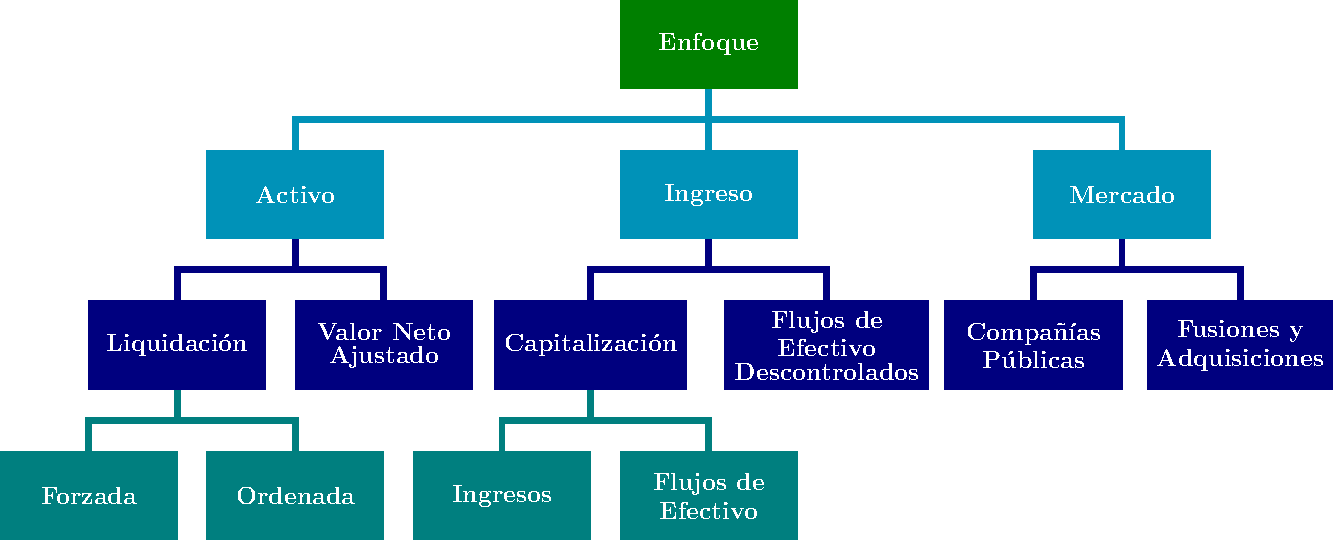
\includegraphics[width=14cm]{\rutaImagenes/enfoques_mas_utilizados_eng}
\end{figure}

\subsubsection{Asset Approach}

The asset approach is a general way to determine the fair value of a company's equity, a business, investment project, tangible asset, or intangible asset using one or more methods based on the value of assets and their net liabilities.\\[10pt]

In business valuation, the asset approach can be considered equivalent to the cost approach in other valuation disciplines. \\[10pt]

There are two general methods in the asset approach for business valuation:\\[10pt]

\textcolor{secundario}{Adjusted Book Value Method:} This method adjusts assets and liabilities (including off-balance sheet items, intangibles, and contingent liabilities) to their market value.\\[10pt]

\textcolor{secundario}{Excess Earnings Capitalization Method:} This method involves a revaluation of all the assets and liabilities of the company. This method is not used to determine the total value of a business but to determine the value of goodwill or intangible assets.\\[10pt]

It is important to distinguish between the application of a valuation method within the asset approach and the ``book value''. Under any valuation standard, the fact that the market value of a business or company is equal to its book value would be a coincidence or would depend on very particular circumstances of the entity being valued.\\[10pt]

\subsubsection{Market Approach}

The market approach determines the fair value of a company's equity, business, investment project, tangible asset, or intangible asset by using methods that compare the appraised asset with similar assets.\\[10pt]

The business, shares, tangible assets, or intangible assets used for comparison should be reasonably similar to the appraised asset. Key factors to consider in determining comparability include:\\[10pt]

\begin{itemize}

\item Sufficient similarity in quantitative and qualitative characteristics.

\item The amount and verifiability of information regarding the asset.

\item Whether the price of the similar asset was determined in a transaction between independent parties, i.e., in a voluntary sale between the parties.

\item Comparisons are generally made using valuation ratios (multiples); the calculation and use of these ratios should provide a significant reference regarding the value of the asset, considering all relevant factors.

\end{itemize}

Methods in the market approach include:\\[10pt]

\textcolor{secundario}{Public Company Guideline Method:} This method determines market multiples of stock prices of publicly traded companies (listed on a stock exchange) with a similar line of business to the appraised company.\\[10pt]

\textcolor{secundario}{Transaction Guideline Method:} This method determines market multiples of similar transactions completed between independent parties.\\[10pt]

\subsubsection{Income Approach}

The income approach is a general way to determine the fair value of a company's equity, business, asset, or intangible asset using one or more methods by which economic benefits are converted into value.\\[10pt]

In the income approach, anticipated benefits are expressed in monetary terms and can be reasonably represented by concepts such as dividends or distributions, various types of earnings, or cash flows.\\[10pt]

To estimate anticipated benefits, elements such as capital structure, historical performance of the entity, the future industry environment, and economic factors must be considered.\\[10pt]

Anticipated benefits are converted into value through procedures that consider expected growth and timing of benefits, as well as the risk profile of the benefits and the time value of money.\\[10pt]

Typically, converting anticipated benefits into value requires determining a capitalization rate or discount rate. To determine these rates, factors such as interest rate levels, expected rates of return by investors in alternative investments, and specific risk characteristics of anticipated benefits must be considered.\\[10pt]







\espacio{7cm}
	
	\begin{center}
 	\printnoidxglossary[type=\acronymtype,title={Acr\'onimos}]
	\printnoidxglossary
	\end{center}
	

\section{DESCRIPCI\'ON DE LOS ENFOQUES DE VALUACI\'ON APLICADOS.}\label{sec:k}

\renewcommand\thefigure{\arabic{figure}} 

%\input{../k.desarrollo_avaluo/k.1.descripcion_enfoques/estimacion_valor_razonable_act_intangible_b}

%\input{../k.desarrollo_avaluo/k.1.descripcion_enfoques/valor_oportunidades_internas}

%\input{../k.desarrollo_avaluo/k.1.descripcion_enfoques/metodologias_de_valuacion_de_negocios_+_intangibles}

%\input{../k.desarrollo_avaluo/k.1.descripcion_enfoques/dcf_intangible}

%\input{../k.desarrollo_avaluo/k.1.descripcion_enfoques/PEERS}

%\input{../k.desarrollo_avaluo/k.1.descripcion_enfoques/enfoque_residual_dinamico}

%\textcolor{secundario}{\gls{rfr}.} El  Flujo de ahorro en Regal\'ias se encuentra mencionado en Bolet\'in C-8 de las Mex NIF como el m\'etodo sugerido para estimar el valor razonable de activos intangibles como marcas, nombres comerciales y otros distintivos similares. Es un modelo de valuaci\'on utilizado para estimar el valor de ciertos activos intangibles  y cuenta con amplia aceptaci\'on en el medio consultor\'ia financiera (\autoref{fig:RFR}).

\begin{figure}[H]
\centering
\caption{Objeto del modelo RFR\label{fig:RFR}}

\includegraphics[width=4cm]{\rutaImagenes/RFR}\\
\end{figure}

\textbf{\textcolor{principal}{Aplicaci\'on del m\'etodo.}} Este modelo involucra la estimaci\'on del valor justo de un activo intangible, cuantificando el valor presente del flujo de pagos de regal\'ias que el propietario del activo intangible est\'a exento (\autoref{fig:RFR_2}). Se basa en la premisa de que el \'unico valor que el comprador de un activo intangible recibe es el ahorro por no tener que pagar regal\'ias a un tercero por el uso de dicho activo.

\begin{figure}[H]
\centering
\caption{Premisas del modelo RFR\label{fig:RFR_2}}
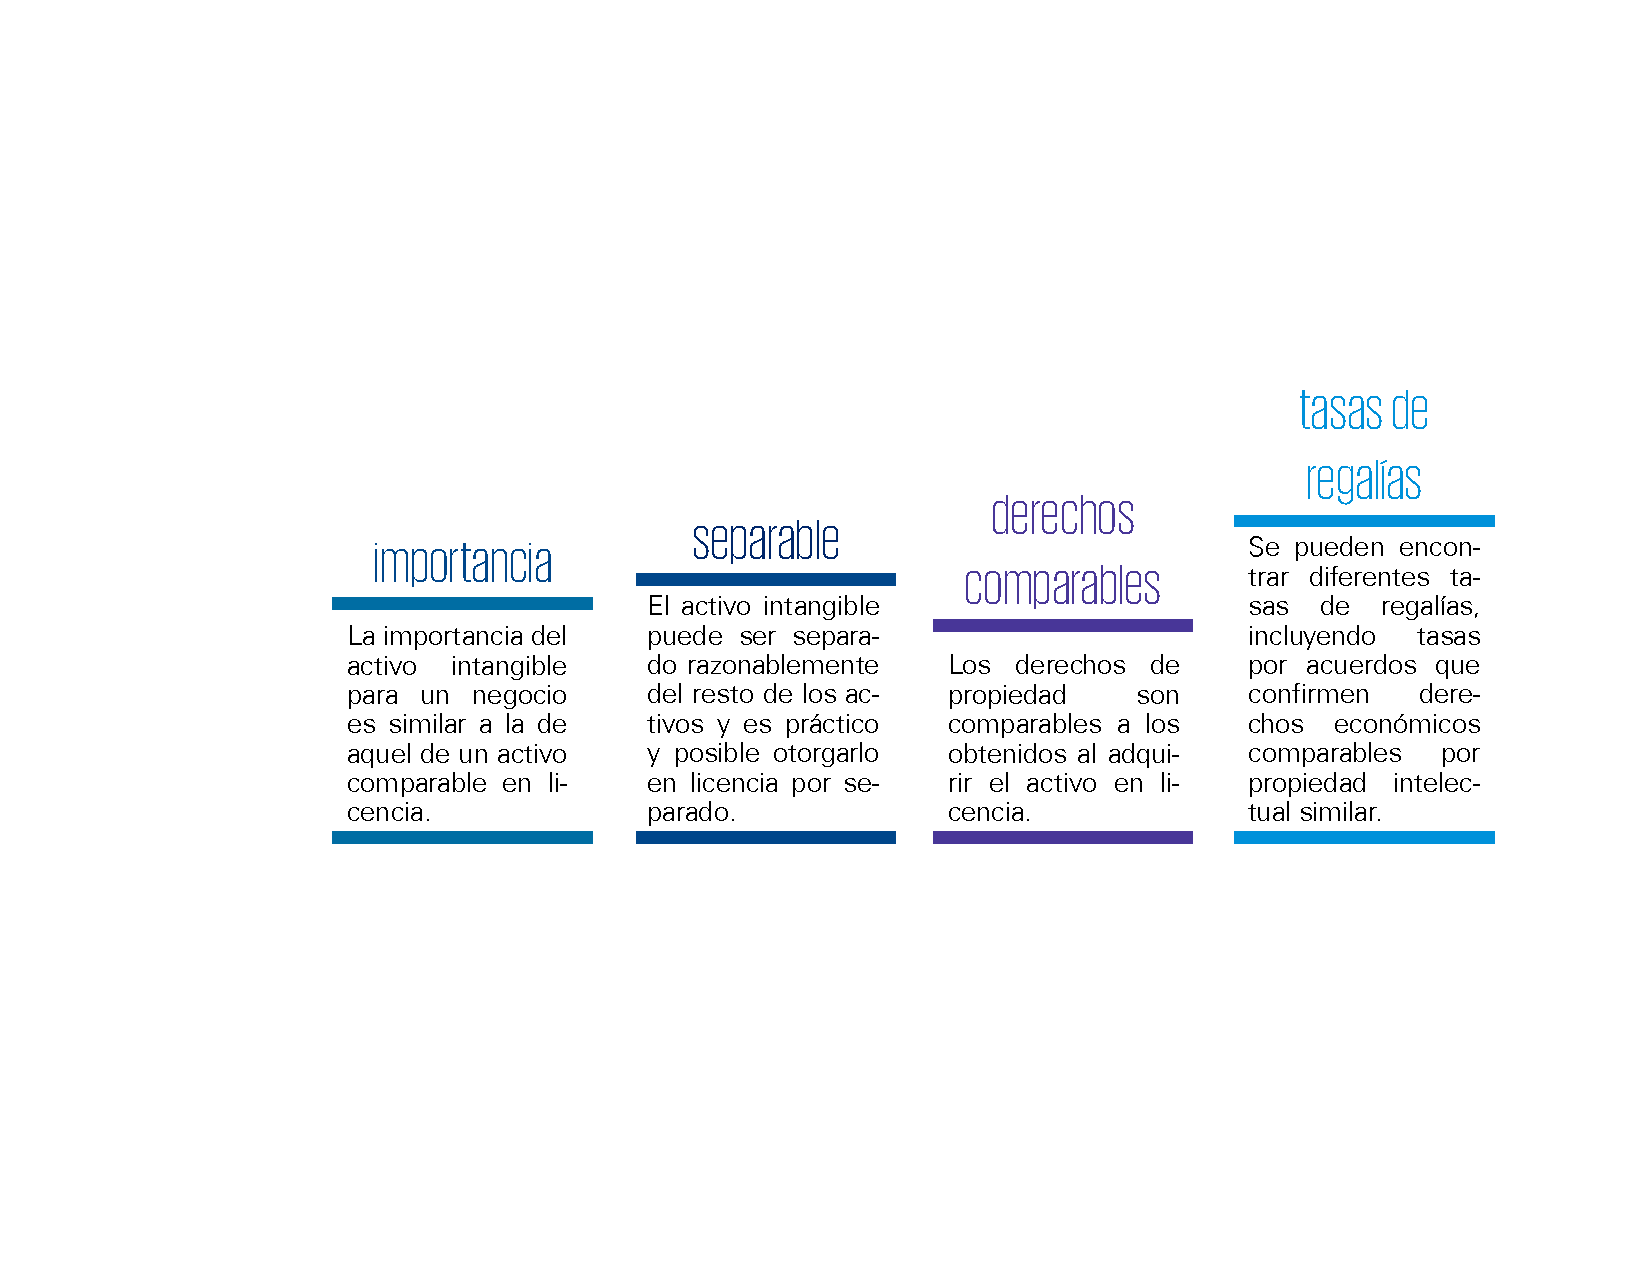
\includegraphics[width=10cm]{\rutaImagenes/RFR_2}\\
\end{figure}


%\input{../k.desarrollo_avaluo/k.1.descripcion_enfoques/estimacion_tasa_desc_intangible}

%\input{../k.desarrollo_avaluo/k.1.descripcion_enfoques/CAPM}

%\input{../k.desarrollo_avaluo/k.1.descripcion_enfoques/estimacion_wacc}


%=================Semblanza======================

%\includepdf[pages=-,pagecommand={\thispagestyle{fancy}}]{../0.semblanza/semblanza}


%-----------------------Desarrollo del avalúo en la especie------------------------------------


%\subsection{DESARROLLO DEL AVAL\'UO EN LA ESPECIE.}\label{sec:k2}

\subsubsection{An\'alisis Financiero}
%Se recibieron los Estados financieros hist\'oricos de \EFde{} y a \EFhasta, por parte del  solicitante, seg\'un se muestran a continuaci\'on:

\begin{figure}[H]
\centering
\caption{Estados de Situaci\'on Financiera Hist\'oricos \EFdeHasta \label{fig:ESF}}
\includegraphics[width=12cm]{../0.imagenes/EF_activo}\\[5pt]

\end{figure}
\begin{figure}[H]
\centering
\includegraphics[width=12cm]{../0.imagenes/EFpasivo_capital}\\

\end{figure}

\begin{figure}[H]
\centering
\caption{Estados de Resultados Hist\'oricos \EFdeHasta \label{fig:ESF}}
\includegraphics[width=12cm]{../0.imagenes/ER}\\
\end{figure}


Para el an\'alisis financiero de dicha empresa, se llevaron a cabo los siguientes m\'etodos:
\begin{enumerate}
\item An\'alisis del Capital Invertido (IC\footnote{Investment Capital}).
\item Razones financieras de liquidez y solvencia (Ratios bancarios).
\item An\'alisis Dupont de 3 elementos.
\item An\'alisis de la Rentabilidad del Capital (ROC\footnote{Return on Capital}).
\item An\'alisis de la Rentabilidad del Capital Operativo Neto (ROIC\footnote{Return on Investment Capital}).
\end{enumerate}

\begin{center}
\underline{An\'alisis del Capital Invertido (IC)}\\[10pt]
\includegraphics[width=12cm]{../0.imagenes/IC}\\[10pt]

\underline{Razones financieras de liquidez y solvencia}\\[10pt]
\includegraphics[width=12cm]{../0.imagenes/ratios}\\[10pt]

\underline{An\'alisis Dupont}\\[10pt]
\includegraphics[width=12cm]{../0.imagenes/dupont}\\[10pt]
\newpage
\underline{An\'alisis ROC}\\[10pt]
\includegraphics[width=12cm]{../0.imagenes/roc}\\[10pt]



\underline{An\'alisis ROIC}\\[10pt]
\includegraphics[width=12cm]{../0.imagenes/roic}\\[10pt]
\end{center}

% \subsubsection{Estimaci\'on de la Tasa de Descuento Ke.}

Cuanto mayor sea el riesgo sistem\'atico de una acci\'on, m\'as elevado ser\'a el rendimiento que los inversionistas esperar\'an de los t\'itulos accionarios. Con la finalidad de estimar una tasa de descuento apropiada en pesos, en t\'erminos nominales y despu\'es de impuestos, se utilizaron los siguientes insumos para determinar el valor de la \gls{wacc}:\\


\textcolor{principal}{Tasa libre de riesgo (Rf).} Se basa en el rendimiento de los bonos gubernamentales, en este caso, se tom\'o en cuenta el pronóstico del rendimiento del \textcolor{principal}{\rfBase}, con el siguiente resultado:

\begin{figure}[H]
\centering
La tasa libre de riesgo obtenida es de \textbf{\rfValor\%}\\[10pt]
 \includegraphics[width=9cm]{\rutaImagenes/banxico/cuadro_1_jul-ago_2023}
\end{figure}

\gls{beta}. Con la finalidad de determinar el factor \gls{beta} apropiado para el negocio, se consider\'o una muestra de mercado de \glspl{leveredbeta} de empresas comparables al negocio valuado:

\textcolor{principal}{Muestra de mercado de la beta del sector,  estructura de Deuda/Capital del sector (D/E), tasa efectiva de impuestos a la utilidad (ETR\%) :}

\espacio{4cm}
\begin{figure}[H]
\centering
\includegraphics[width=6cm]{../0.imagenes/beta_1}\\
\end{figure}

La beta apalancada de sector que corresponde a la empresa es de \textcolor{principal}{\textbf{\valorBeta x }(mediana)}\\

F\'ormula de BETA Despalancada:
\begin{figure}[H]
\centering

\includegraphics[width=8cm]{\rutaImagenes/beta_apalancada}
\end{figure}

El valuador llev\'o a cabo la estimaci\'on del pron\'ostico de BETA desapalancada al negocio, habiendo aplicado a la proporci\'on de deuda/capital del sujeto, el promedio de la muestra y la tasa fiscal efectiva del sector (ETR\footnote{Efective Tax Rate}); con un resultado de \textcolor{principal}{\betaDesapalancada x}.\\

F\'ormula de BETA Reapalancada:\\

\begin{figure}[H]
\centering

\includegraphics[width=8cm]{\rutaImagenes/beta_reapalancada}
\end{figure}

Una vez obtenido el indicador de BETA desapalancada del sector, el valuador llev\'o a cabo la estimaci\'on del pron\'ostico de BETA reapalancada al negocio sujeto de valuaci\'on, habiendo aplicado a la proporci\'on de deuda/capital del sujeto, la mediana\footnote{Conforme a la aplicaci\'on del rango intercuartil como medida de estandarizaci\'on}  de la muestra del sector y la tasa fiscal de M\'exico (MTR\footnote{Marginal Tax Rate}), con un resultado de \textcolor{principal}{\betaReapalancada x}\\



\textcolor{principal}{Prima de riesgo del mercado de capitales}. Se obtuvo del promedio hist\'orico de la diferencia de rendimientos o ``\textit{spread}'' entre el mercado accionario \mercadoAccionario{} mediante el indicador conocido como el \gls{erp} (\textit{enterprise risk premium}).\\

\begin{figure}[H]
\centering
La prima de riesgo de mercado (\gls{erp}) es de \textbf{\textcolor{principal}{\erpValor\%}} \\[10pt]

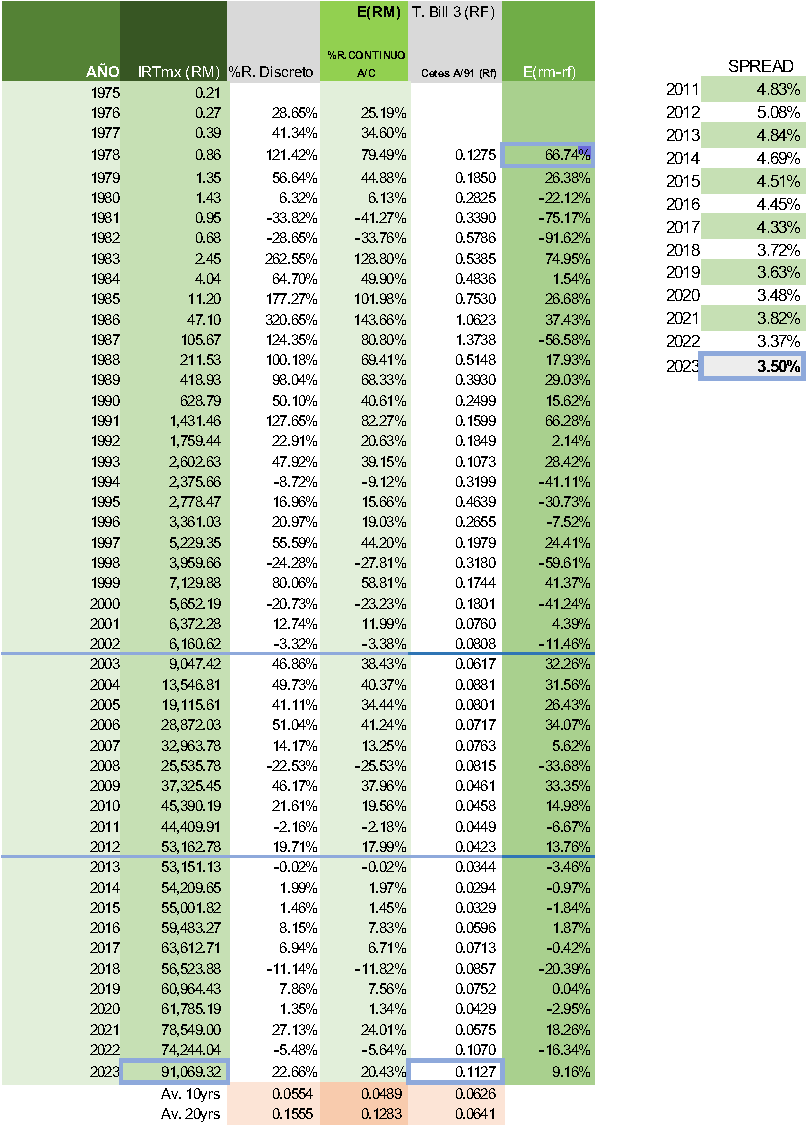
\includegraphics[width=5cm]{../0.imagenes/erp}
\end{figure}

%\textcolor{principal}{Riesgo Pa\'is (\gls{crp}).} Corresponde al riesgo pa\'is de M\'exico, seg\'un indicador de JP Morgan. Se considera un pron\'ostico para la prima de riesgo adicional de \crpValor{} puntos base.
%
%\begin{figure}[H]
%\centering
%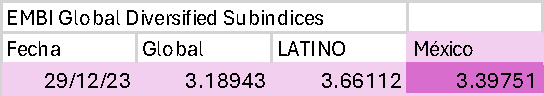
\includegraphics[width=8cm]{../0.imagenes/crp}
%\end{figure}

\textcolor{principal}{Prima por tamaño (\textit{Size Prime}).} \\[5pt]

Se tomo una prima por tamaño para la firma, a partir del valor en libros del capital contable de acuerdo a la siguiente tabla.\\

\textit{Nota. La tabla muestra la prima por tamaño a partir del valor en libros del capital contable en Millones de Euros.% Considerando el tipo de cambio  MEX/EUR a la fecha de valores de 20.8560 se obtiene un capital en euros por EUR 24,451,811.08.}
}

\begin{figure}[H]
\centering
La prima de tamaño es de \textbf{\textcolor{principal}{\sizePrime\%}} \\
\includegraphics[width=.8\textwidth]{../0.imagenes/size_prime_2}
\end{figure}


Estimaci\'on del costo de capital (\gls{ke}), con un resultado de \textcolor{principal}{\keValor\%.}

\begin{figure}[H]
\centering
\includegraphics[width=10cm]{../0.imagenes/ke}
\end{figure}


\textcolor{principal}{Costo de la deuda (\gls{kd}).} Para determinar la tasa \gls{wacc}, se consider\'o el costo impl\'icito de la deuda de la organizaci\'on, de acuerdo a par\'ametros de mercado de empresas similares:

\begin{figure}[H]
\centering
\includegraphics[width=10cm]{../0.imagenes/kd}
\end{figure}

\textcolor{principal}{C\'alculo del \gls{wacc}.} Como resultado de las consideraciones anteriores, se estima una \gls{wacc} en t\'erminos nominales y despu\'es de impuestos de \textcolor{principal}{\waccValor\%}.\\

\begin{figure}[H]
\centering
\includegraphics[width=12cm]{../0.imagenes/wacc}
\end{figure}



%\subsection{Desarrollo DCF}

\textcolor{principal}{An\'alisis Hist\'orico de los Ingresos y Flujos operativos del Negocio.}\\

El perito valuador llev\'o a cabo el an\'alisis financiero de los ingresos (\textit{Revenues}) y de la utilidad operativa del negocio (Ebit) del periodo de \EFdeHasta, con el objetivo de usar de base dicho an\'alisis para proyectar correctamente los flujos de operaci\'on de la sociedad en la aplicaci\'on del modelo DCF como m\'etodo principal para determinar el valor razonable de la firma.

\begin{figure}[H]
\centering
\includegraphics[width=14cm]{../0.imagenes/dcf_1}
\end{figure}

\begin{figure}[H]
\centering
\includegraphics[width=8cm]{../0.imagenes/dcf_2}
\end{figure}


\textcolor{principal}{\textbf{PROYECCI\'ON FINANCIERA.} Proyecci\'on de Ingresos y del Flujo de Operaci\'on del Negocio.} El perito valuador llev\'o a cabo la proyecci\'on del EBIT de la sociedad del periodo \periodoProyeccion. Como premisas de la proyecci\'on se utilizaron los siguientes indicadores (\textit{ceteris paribus}): i) \gls{cagr} \periodoProyeccion: \proyCagr\%, ii) Margen Operativo (\textit{Ebit margin}): \proyEbitMargin\%.

\begin{figure}[H]
\centering
\includegraphics[width=15cm]{../0.imagenes/dcf_proy}
\end{figure}

\textbf{\textcolor{principal}{Estimaci\'on del Flujo de Efectivo Libre a la Firma (\gls{fcff}).}} El valuador llev\'o a cabo la estimaci\'on del Flujo de Caja Libre a la firma
%, conforme a la metodolog\'ia conocida como ``Ebit sintetizado'', la cual estima dos premisas: i) El flujo de operaci\'on neto o \gls{nopat} (INFLOWS) y  ii) Los cambios al capital invertido (OUTFLOWS)
. Dicha estimaci\'on representa la capacidad de la empresa de generar flujo de efectivo con sus activos operativos. La productividad de un activo se mide en funci\'on de la capacidad de generar rentabilidad para sus accionistas y fondeadores.\\

Se utilizaron las siguientes premisas (\textit{ceteris paribus}): i) Tasa fiscal efectiva (\gls{etr}): \tasaFiscal\%, ii) Tasa de Reinversi\'on (\textit{Reinvestment Rate}): \reinvestmentRate\%. Los resultados de la proyecci\'on se detallan a cotinuaci\'on:

\begin{figure}[H]
\centering
\includegraphics[width=15cm]{../0.imagenes/FCFF}
\end{figure}



\textcolor{principal}{OBTENCI\'ON DEL INDICADOR DE VALOR DE LA FIRMA Y DEL NEGOCIO MEDIANTE EL M\'ETODO DCF.} Se analiz\'o el modelo explicado, el cual cuenta con amplia aceptaci\'on en la valuaci\'on de negocios a nivel mundial.  Sus resultados se exhiben a continuaci\'on:

\begin{figure}[H]
\centering
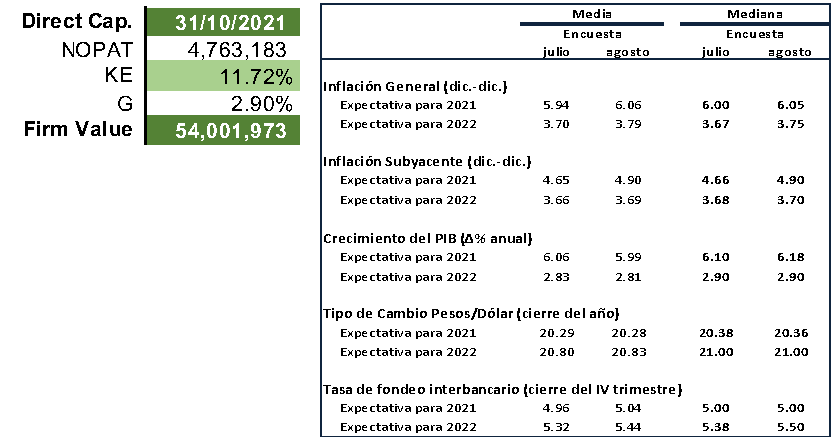
\includegraphics[width=14cm]{../0.imagenes/valor_dcf}\\
\textcolor{principal}{\textbf{\textbullet Valor razonable del negocio en marcha: \$\valorDCF{}MXN}}
\end{figure}


%\subsubsection{RELATIVE VALUATION METHOD.}

\textcolor{principal}{Market Sample of Trading Multiples  (PEERS))}. The market approach was applied based on an indicator known as ``\textcolor{principal}{\peersa} x''; with an estimate of \textcolor{principal}{\peersaMult x} \footnote{\peersaEst{} of the sample} times \peersaTo:\\


%\begin{figure}[H]
%\centering
%
\includegraphics[width=11cm]{../0.imagenes/peers_1}
%\end{figure}

The market approach was also applied based on an indicator known as ``\textcolor{principal}{\peersb} x''; with an estimate of  \textcolor{principal}{\peersbMult x} \footnote{\peersbEst{} of the sample} times \peersbTo:\\

\begin{figure}[H]
\centering

\includegraphics[width=14cm]{../0.imagenes/peers_1}
\end{figure}

%\newpage
%
%Se aplic\'o el enfoque de mercado con base en un indicador conocido como ``\textcolor{principal}{\peersc} x''; con una estimaci\'on de \textcolor{principal}{\peerscMult x} \footnote{\peerscEst{} de la muestra} veces \peerscTo:\\
%
%\begin{figure}[H]
%\centering
%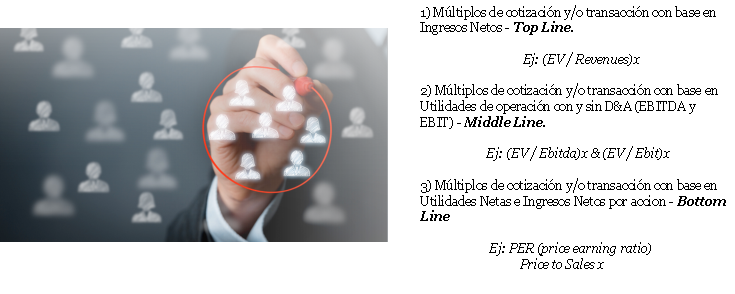
\includegraphics[width=11cm]{../0.imagenes/peers_3}
%\end{figure}
%
%\newpage
%
%Se aplic\'o el enfoque de mercado con base en un indicador conocido como ``\textcolor{principal}{\peersd} x''; con una estimaci\'on de \textcolor{principal}{\peersdMult x} \footnote{\peersdEst{} de la muestra} veces \peersdTo:\\
%
%\begin{figure}[H]
%\centering
%\includegraphics[width=11cm]{../0.imagenes/peers_4}
%\end{figure}
%
%\newpage
%
%Se aplic\'o el enfoque de mercado con base en un indicador conocido como ``\textcolor{principal}{\peerse} x''; con una estimaci\'on de \textcolor{principal}{\peerseMult x} \footnote{\peerseEst{} de la muestra} veces \peerseTo:\\
%
%\begin{figure}[H]
%\centering
%\includegraphics[width=11cm]{../0.imagenes/peers_5}
%\end{figure}



\subsection{Value of the Business by PEERS.} The appraiser conducted a capitalization by multiples for the estimation of the fair value of the company, according to the market approach; as can be seen:

\begin{figure}[H]
\centering
\includegraphics[width=.7\textwidth]{../0.imagenes_eng/valor_peers}\\

%Valor razonable por PEERS: \textcolor{principal}{\$\valorPeers MXN}
\end{figure}

%
\newcommand{\ponda}{Direct Capitalization)}
\newcommand{\pondaPorcentage}{33}
\newcommand{\pondb}{\peersa}
\newcommand{\pondbPorcentage}{33}
\newcommand{\pondc}{\peersb}
\newcommand{\pondcPorcentage}{33}
\newcommand{\pondd}{\peersd}
\newcommand{\ponddPorcentage}{30}
\newcommand{\ponde}{\peersd}
\newcommand{\pondePorcentage}{30}

\subsection{WEIGHTED FAIR VALUE OF THE ONGOING BUSINESS, WITH FIGURES AS OF \fechaValoresCorto.}


The fair value of the firm (Firm Value), as of the valuation date, is concluded next, having given the following importance to the models in the weighting: i) A weight of \pondaPorcentage\% to the valuation model known as \ponda{}, ii) A weight of \pondbPorcentage\%  to the relative valuation model (PEERS) known as \pondb{} x; iii) A weight of \pondcPorcentage\%  to the relative valuation model (PEERS) known as \pondc{} x; as shown below:

\begin{figure}[H]
\centering
\includegraphics[width=12cm]{../0.imagenes_eng/valor_ponderado_firma}\\

\textbf{\textcolor{principal}{Firm Value as of  \fechaValoresCorto:} \$\valorFirma{} MXN}\\[5pt]
(\textcolor{principal}{\valorFirmaLetra{} pesos 00/100 M.N.})
\end{figure}


%%\newcommand{\valorCapitalM}{906}
%\newcommand{\valorCapitalm}{356}
%\newcommand{\valorCapitalc}{853}
%\newcommand{\valorCapital}{\valorCapitalM,\valorCapitalm,\valorCapitalc}
%\newcommand{\valorCapitalLetra}{\Numberstringnum{\valorCapitalM}{} millones, \numberstringnum{\valorCapitalm}{} mil, \numberstringnum{\valorCapitalc}}

\subsection{FAIR VALUE OF EQUITY CAPITAL, WITH FIGURES AS OF \fechaValoresCorto}

Once the value of the business firm was estimated, the appraiser proceeded to subtract the Net Debt of the business, thus obtaining the fair value of the equity capital.\\

Next, the fair value of the equity capital (\textit{\gls{equityvalue}}) as of the valuation date is concluded:\\


\begin{figure}[H]
\centering
\textbf{\textcolor{principal}{Equity Capital Value as of \fechaValoresCorto:} \$\valorCapital{} MXN}\\
\includegraphics[width=8cm]{../0.imagenes_eng/valor_cap_acc}\\
(\textcolor{principal}{\valorCapitalLetra{} pesos 00/100 M.N.})


\end{figure}


%\subsection{VALUACI\'ON DE ACTIVOS INTANGIBLES}

%\input{../k.desarrollo_avaluo/k.2.desarrollo_avaluo/desarrollo_rfr}

%\subsection{VALOR RAZONABLE PONDERADO DE LOS ACTIVOS INTANGIBLES VALUADOS.}

Despu\'es de haberse realizado el an\'alisis de valor del negocio en marcha con sus activos intangibles, conforme a la aplicaci\'on de los modelos financieros descritos en este presente cap\'itulo, el valuador llev\'o a cabo como parte de su an\'alisis conclusivo, la ponderaci\'on de los dos modelos: i) Residual din\'amico por \gls{dcf} (50\%), ii) Flujo de Ahorro en Regal\'ias (\gls{rfr}) (50\%):

\begin{figure}[H]
\centering
\includegraphics[width=9cm]{../0.imagenes/valor_pond_activo_intangible}\\[10pt]

\textbf{\textcolor{principal}{Valor del Activo Intangible al \fechaValoresCorto:} \$\valorActivoIntangible{} \monedaCode}\\[5pt]
(\textcolor{principal}{\valorActivoIntangibleLetra{} \moneda{} 00/100 M.N.})


\end{figure}






%-----------------------CONSIDERACIONES PREVIAS A LA CONCLUSI\'ON------------------
\section{CONSIDERACIONES PREVIAS A LA CONCLUSI\'ON}\label{sec:o}

\begin{enumerate}[a.]

\item Para la realización del presente avalúo, como se indicó con anterioridad, se tomó como base la información y documentación proporcionada por el solicitante y se realizó el estudio.

\item Se obtuvo el resultado que más adelante se indica, de acuerdo a todos los cálculos estimados con las metodologías de valuación aplicadas y conforme a las reglas de valuación.

\item Para la realización de la presente estimación de valor, se consideraron los documentos exhibidos por el solicitante, mismos que han quedado descritos en el presente dictamen valuatorio, así como el dicho de los solicitantes.

\item La posesión de este avalúo, o la obtención de una copia, no conllevan el derecho a su publicación parcial o total, y no podrá ser usada para propósitos personales u otros distintos a los establecidos en el uso del presente avalúo.

\item Las estimaciones realizadas por los suscritos Peritos Valuadores derivan de las condiciones generalmente aceptadas para este tipo de trabajos. Este documento no es predicción del futuro. Los suscritos Peritos Valuadores no pueden garantizar que dichos pronósticos y estimaciones se materializarán.

\item No existe responsabilidad alguna por parte de los suscritos Peritos Valuadores por actualizar este avalúo por eventos o circunstancias que ocurran con posterioridad a la fecha del mismo.

\item El presente estudio sólo es válido para el propósito y objeto que se indica en los antecedentes y cuando cuente con la firma de los valuadores.

\item Los suscritos Peritos Valuadores que firman no tienen interés presente o futuro en la propiedad que es objeto de este informe, ni tampoco tiene intereses personales o parcialidad con respecto a las partes involucradas.

\item Este dictamen valuatorio sólo podrá ser usado íntegro y no en partes. Ninguna parte del reporte podrá ser utilizada en conjunto a algún estudio ajeno al mismo. La publicación del mismo o cualquiera de sus partes, sin la autorización escrita de los suscritos Peritos Valuadores está prohibida. Este avalúo no podrá ser usado por ninguna persona o entidad distinta a la que esté dirigida o para un propósito o fin distinto al estipulado. 

\item El presente dictamen forma parte de un estudio mayor, cuyos cálculos y papeles de trabajo no se anexan al mismo. 

\item El presente estudio no valida o señala su tratamiento contable y fiscal, conforme a las normas de información financiera (NIF), la ley del ISR, la ley del IVA y demás normatividad aplicable.

\item El presente documento no puede considerarse como un reporte de auditoría o de \textit{due diligence}. Tampoco puede considerarse que el presente trabajo es resultado de una asesoría en materia fiscal, contable, financiera, jurídica o corporativa.

\item Los solicitantes declararon, bajo protesta de decir verdad, (i) que todos los documentos que fueron entregados para la realización de este dictamen son verdaderos, y que los mismos corresponden a la realidad; (ii) que todas la declaraciones realizadas por ellos a los suscritos peritos valuadores y a su equipo son ciertas y verdaderas; y (iii) que ha leído con detenimiento y cuidado el dictamen valuatorio, y expresa su acuerdo y consentimiento respecto de todas y cada una de sus partes. De esta forma, el uso del presente dictamen corresponde a una aceptación tácita sobre el contenido del mismo.

\end{enumerate}

\espacio{7cm}
\section{CONCLUSIONES.}\label{cap:6}
\thispagestyle{fancy}
%-----------------------CONCLUSIÓN DE LA VALUACIÓN-----------------------

\subsection*{CONCLUSI\'ON DE LA VALUACI\'ON.}\label{sec:p}
\textcolor{principal}{\underline{UNICA.-}} El \textcolor{principal}{VALOR RAZONABLE} de la sociedad \textcolor{principal}{\empresaSolicitante} como negocio en marcha (\textit{\gls{firmvalue}}), as\'i como de su capital accionario (\gls{equityvalue}) conforme a la aplicaci\'on de los modelos de valuaci\'on descritos en los cap\'itulos \ref{cap:4} y \ref{cap:5}  de este dictamen, con fecha de valores al \fechaValores, seg\'un el prop\'osito y uso del aval\'uo, es por la siguiente cantidad:\\

\begin{figure}[H]
\centering
\textcolor{principal}{Valor de la Firma al \fechaValoresCorto:}\textbf{\$\valorFirma{} \monedaCode}\\

(\textcolor{secundario}{\valorFirmaLetra{} \moneda{} 00/100 M.N.})

\includegraphics[width=12cm]{../0.imagenes/valor_ponderado_firma}\

\textcolor{principal}{Valor del Capital Accionario al \fechaValoresCorto:} \textbf{\$\valorCapital{} \monedaCode}\\
(\textcolor{secundario}{\valorCapitalLetra{} \moneda{} 00/100 M.N.})\\
\end{figure}

\begin{figure}[H]
\centering
\includegraphics[width=7.5cm]{../0.imagenes/valor_cap_acc}

\end{figure}
\espacio{.5cm}

\vspace{2cm}

A nuestro mejor juicio y parecer, siendo los \textcolor{principal}{ \diainforme{} d\'ias del mes de \monthname[\mesinforme]{} del a\~no \annoinforme{} (\numberstringnum{\annoinforme})} seg\'un el criterio valuatorio explicado en el desarrollo de este dictamen, expedimos el presente \textcolor{principal}{DICTAMEN VALUATORIO}, con \textcolor{principal}{\textbf{FECHA DE VALORES}} al d\'ia \textcolor{principal}{\textbf{\fechaValores}}; para todos los efectos a que haya lugar.\\

Por todo lo cual y con fundamento en el artículo 6$^\circ$ fracción II de la Ley Federal de Correduría Pública y el artículo 56 bis de su Reglamento, para los efectos legales a que hubiera lugar, rindo el presente avalúo y lo expido debidamente en la Ciudad de México, hoy día de su fecha, \diainforme{}  (\numberstringnum{\diainforme}) de \monthname[\mesinforme] de \annoinforme (\numberstringnum{\annoinforme}).



\begin{table}[H]
\centering
	\begin{tabular}{cm{1cm}c}
	\begin{minipage}{7cm}
	\begin{center}
		JOSÉ RAMÓN CLARK GUZMÁN,
		Corredor Público número 81 de la
		Ciudad de México, expido el presente
		dictamen valuatorio.\\[1cm]
		
		\rule{7cm}{.4pt}\\
		JOSÉ RAMÓN CLARK GUZMÁN
		
		
	\end{center}
	\end{minipage}&&
	\begin{minipage}{7cm}
	\begin{center}
		PERITO AUXILIAR\\[1cm]
		
		\rule{7cm}{.4pt}\\
		DIEGO MIGUEL\\
		PEREZCANO BELTRÁN
		%\nombreAuxiliar\\
		%\textcolor{principal}{\descripcionFirmaAuxiliar}
		
	\end{center}
	\end{minipage}
	
	\end{tabular}
\end{table}


%----------------------REPORTE FOTOGRAFICO------------------------------
\section{REPORTE FOTOGR\'AFICO}\label{sec:q}
No Aplica.
%---------------------ANEXOS-------------------------------------------------------- 
\section{ANEXOS}\label{sec:r}




\label{lastpage}
\end{document}
